% Created 2022-10-15 Sat 13:37
% Intended LaTeX compiler: pdflatex
\documentclass[11pt]{article}
\usepackage[utf8]{inputenc}
\usepackage[T1]{fontenc}
\usepackage{graphicx}
\usepackage{grffile}
\usepackage{longtable}
\usepackage{wrapfig}
\usepackage{rotating}
\usepackage[normalem]{ulem}
\usepackage{amsmath}
\usepackage{textcomp}
\usepackage{amssymb}
\usepackage{capt-of}
\usepackage{hyperref}
\author{Max Jauregui}
\date{\today}
\title{Finanças pessoais 2022}
\hypersetup{
 pdfauthor={Max Jauregui},
 pdftitle={Finanças pessoais 2022},
 pdfkeywords={},
 pdfsubject={},
 pdfcreator={Emacs 27.1 (Org mode 9.3)}, 
 pdflang={Pt_Br}}
\begin{document}

\maketitle
\setcounter{tocdepth}{2}
\tableofcontents


\section{Análise mensal}
\label{sec:org8afaf8c}

\subsection{Outubro}
\label{sec:org8bfed6d}

\subsubsection{Saldo anterior}
\label{sec:org33a9aec}

O saldo anterior nas contas bancárias é R\$ 3472.72

\subsubsection{Tabela de gastos e ingressos}
\label{sec:org94e4375}

\begin{center}
\begin{tabular}{rlrl}
Data & Descrição & Valor & Forma\\
\hline
2022-10-01 & Padaria & 16.63 & Crédito\\
2022-10-01 & Cafeteria & 37.52 & Crédito\\
2022-10-02 & Restaurante & 79.80 & Crédito\\
2022-10-03 & Mercado & 212.80 & Crédito\\
2022-10-05 & Trade & 109.34 & Depósito\\
2022-10-06 & Condomínio & 432.03 & Débito\\
2022-10-08 & Combustível & 80.00 & Crédito\\
2022-10-10 & Cartão & 478.00 & Débito\\
2022-10-11 & Energia & 44.14 & Débito\\
2022-10-11 & Internet & 99.90 & Débito\\
2022-10-14 & Aluguel & 704.00 & Débito\\
\end{tabular}
\end{center}

\subsubsection{Classificação por forma de pagamento}
\label{sec:org7f37fd5}

\textbf{Crédito:} Gastos realizados usando cartão de crédito

\textbf{Débito:} Gastos realizados via PIX, pagamento de boleto, transferência bancária ou cartão de débito.

\textbf{Depósitos:} Ingressos de fontes diversas.

\begin{center}
\begin{tabular}{lr}
 & Valor\\
\hline
Crédito & 426.75\\
Depósito & 109.34\\
Débito & 1758.07\\
\end{tabular}
\end{center}

\begin{center}
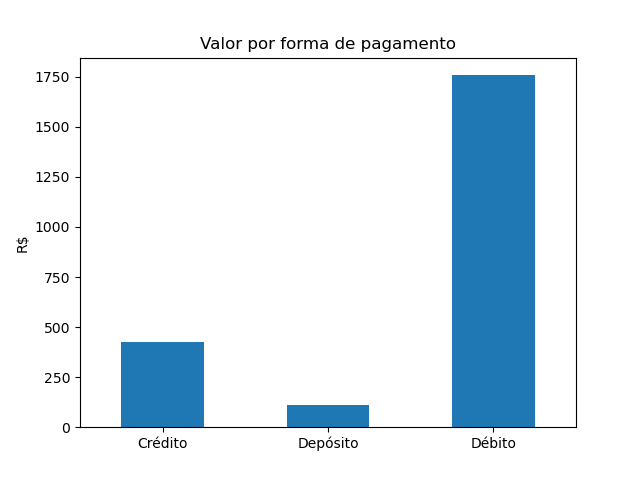
\includegraphics[width=.9\linewidth]{outubro-forma.png}
\end{center}

\subsubsection{Classificação dos gastos e ingressos}
\label{sec:orga9ab4b4}

\begin{center}
\begin{tabular}{lr}
 & Valor\\
\hline
Açougue/Mercado/Padaria & 229.43\\
Fatura do cartão & 478.00\\
Moradia & 1280.07\\
Renda extra & 109.34\\
Restaurante/Cafeteria & 117.32\\
Transporte & 80.00\\
\end{tabular}
\end{center}

\begin{center}
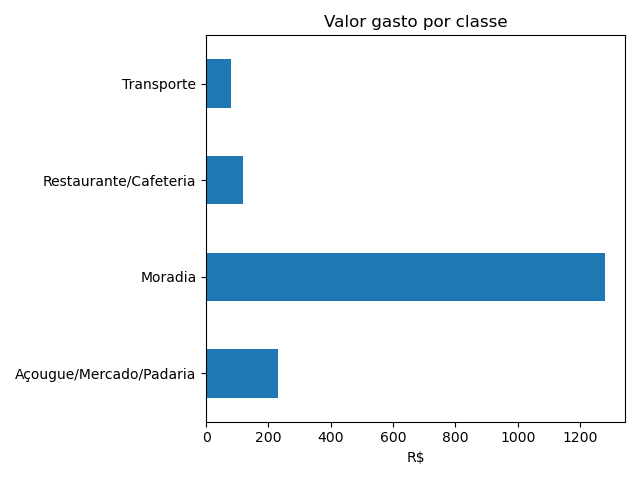
\includegraphics[width=.9\linewidth]{outubro-classe.png}
\end{center}

\subsubsection{Saldo posterior}
\label{sec:orgc3992e5}

O saldo posterior nas contas bancárias é R\$ 1823.99
\end{document}